\chapter{Indexed methods}
\label{chr:index}

Suffix trees are elegant data structures but they are rarely used in practice.
Although suffix trees provides theoretically optimal construction and query time, their high space consumption prohibits practical applicability to large string collections.
A practical study on suffix trees \citep{Kurtz1999} reports that efficient implementations achieve sizes between $12~n$ and $20~n$ bytes per character.
For instance, two years before completing the sequencing of the human genome, \citeauthor{Kurtz1999} conjectured the resources required for computing the suffix tree for the complete human genome (consisting of about $3 \cdot 10^9$~bp) in 45.31~GB of memory and nine hours of CPU time, and concluded that \emph{``it seems feasible to compute the suffix tree for the entire human genome on some computers''}.

One might be tempted to think that such memory requirements are not anymore a limiting factor as, at the time of writing, even standard personal computers come with 32~GB of main memory.
Indeed, over the last decades, the semiconductors industry followed the exponential trends dictated by Moores' law and yielded not only exponentially faster microprocessors but also larger memories.
Unfortunately, memory latency improvements have been more modest, leading to the so called memory wall effect \citep{Wilkes1995}: data access times are taking an increasingly fraction of total computation times.
Thus, if in \citeyear{Knuth1973} \citeauthor{Knuth1973} wrote that \emph{``space optimization is closely related to time optimization in a disk memory''}, forty years later one can simply say that space optimization is always related to time optimization.

Over the last years, a significant effort has been devoted to the engineering of more space-efficient data structures to replace the suffix tree in practical applications.
In particular, much research has been done into designing succinct (or even compressed) data structures providing efficient query times using space proportional to that of the uncompressed (or compressed) input.
Thanks to this research, the human genome can be indexed in as little as 3.5~GB of memory without affecting query time in respect to classic indices.

In this chapter, I introduce some classic full-text indices (suffix arrays and $q$-gram indices) and subsequently succinct full-text indices (uncompressed FM-index variants).
Afterwards, I expose generic string matching algorithms, working on any of these data structures, and at the same time provide their experimental evaluation.
My implementation of all these algorithms and data structures is publicly available in source form within the \CC library SeqAn \citep{Doering2008}.

\section{Classic full-text indices}

\subsection{Suffix array}

The key idea of the suffix array \citep{Manber1990} is that most information explicitly encoded in a suffix trie is superfluous for string matching.
The explicit representation of suffix trie's internal nodes and outgoing edges can be omitted.
Leaves pointing to the sorted suffixes are sufficient to perform exact string matching or even top-down traversals.
Indeed, any path from the root to an internal node is computed on the fly via binary search over the leaves.
In this way, an additional logarithmic time complexity is paid to reduce space consumption by a linear factor.
I formally define the (generalized) suffix array and later show how to emulate suffix trie traversals.

\begin{definition}
The \emph{suffix array} of a padded string $s$ of length $n$ is an array $A$ containing a permutation of the interval $[1,n]$, \st $s_{A[i] \dots n} <_{lex} s_{A[i+1] \dots n}$ for all $1 \leq i < n$.
\end{definition}

\begin{definition}
The \emph{generalized suffix array} of a padded string collection $\Sc$ (definition~\ref{def:coltd}), consisting of $c$ strings of total length $n$, is an array $A$ of length $n$ containing a permutation of all pairs $(i,j)$ where $i$ points to a string $s^i \in \Sc$ and $j$ points to one of the $n_i$ suffixes of $s^i$.
Pairs are ordered \st $\Sc_{A[i] \dots} <_{lex} \Sc_{A[i+1] \dots}$ for all $1 \leq i < n$.
\end{definition}

\begin{figure}[b]
\begin{center}
\caption[Example of (generalized) suffix array]{(Generalized) suffix array. (\subref{fig:sa}) Suffix array of the string {\ttfamily ANANAS\$}. (\subref{fig:gsa}) Generalized suffix array of the string collection $\Sc = \{$ {\ttfamily ANANAS$\$_1$}, {\ttfamily CACAO$\$_2$} $\}$.}

\begin{subfigure}[t]{0.45\textwidth}
\begin{center}
\caption[Example of suffix array]{Suffix array.}
\label{fig:sa}
\ttfamily
\begin{tabular}{ccl}
$i$ & $A[i]$ & $s_{A[i]\dots n}$\\
\midrule
1 & 7 & \$\\
2 & 1 & ANANAS\$\\
3 & 3 & ANAS\$\\
4 & 5 & AS\$\\
5 & 2 & NANAS\$\\
6 & 4 & NAS\$\\
7 & 6 & S\$\\
\end{tabular}
\end{center}
\end{subfigure}%
\begin{subfigure}[t]{0.45\textwidth}
\begin{center}
\caption[Example of generalized suffix array]{Generalized suffix array.}
\label{fig:gsa}
\ttfamily
\begin{tabular}{rcl}
$i$ & $A[i]$ & $\Sc_{A[i]\dots}$\\
\midrule
1 & (1,7) & $\$_1$\\
2 & (2,6) & $\$_2$\\
3 & (2,2) & ACAO$\$_2$\\
4 & (1,1) & ANANAS$\$_1$\\
5 & (1,3) & ANAS$\$_1$\\
6 & (2,4) & AO$\$_2$\\
7 & (1,5) & AS$\$_1$\\
8 & (2,1) & CACAO$\$_2$\\
9 & (2,3) & CAO$\$_2$\\
10 & (1,2) & NANAS$\$_1$\\
11 & (1,4) & NAS$\$_1$\\
12 & (2,5) & O$\$_2$\\
13 & (1,6) & S$\$_1$\\
\end{tabular}
\end{center}
\end{subfigure}

\end{center}
\end{figure}

The suffix array is constructed in $\Oh(n)$ time, for instance using the \citep{Kaerkkaeinen2003} algorithm, or using non-optimal but practically faster algorithms, \eg \citep{Schuermann2007}.
The space consumption of the suffix array is $n \log{n}$ bits.
When $n < 2^{32}$, a 32 bit integer is sufficient to encode any value in the range $[1,n]$.
Consequently, the space consumption of suffix arrays for texts shorter than 4~GB is $4 n$ bytes.

\citeauthor{Weese2013} gives a generalization of \citeauthor{Kaerkkaeinen2003} algorithm to construct the generalized suffix array in $\Oh(n)$ time.
The space consumption of the generalized suffix array is $n \log{cn^*}$ bits, where $n^* = \max{\,n_i}$.
For instance, the human genome GRCh38 is a collection of 24 sequences, among whose the largest one consists of 248~Mbp.
Hence, to represent the generalized suffix array of GRCh38 I use pairs of $1+4$~bytes.
The suffix array of GRCh38 fits in 15~GB of memory and is constructed in about one hour on a modern computer \citep{Weese2013}.

\begin{figure*}[t!]
\begin{minipage}[t]{.5\textwidth}
\begin{algorithm}[H]
\Algorithm{L}{$\Tn,c$}
\begin{tabular}{ll}
\textbf{Input}  & $\Tn$ : pointer to a suffix array node\\
				& $c$ : character to query\\
\textbf{Output} & integer denoting the left interval\\
\end{tabular}
\begin{algorithmic}[1]
\State {$l_1 \gets \Tn.l$}
\State {$l_2 \gets \Tn.r$}
\While {$l_1 < l_2$}
	\State {$i \gets \lfloor \frac{l_1+l_2}{2} \rfloor$}
	\If {$\Sc_{A[i] + \Tn.d} <_{lex} c$}
		\State {$l_1 \gets i+1$}
	\Else
		\State {$l_2 \gets i$}
	\EndIf
\EndWhile
\State \Return $l_1$
\end{algorithmic}
\label{alg:sa-lower}
\end{algorithm}
\end{minipage}
\hfill
\begin{minipage}[t]{.5\textwidth}
\begin{algorithm}[H]
\Algorithm{R}{$\Tn,c$}
\begin{tabular}{ll}
\textbf{Input}  & $\Tn$ : pointer to a suffix array node\\
				& $c$ : character to query\\
\textbf{Output} & integer denoting the right interval\\
\end{tabular}
\begin{algorithmic}[1]
\State {$r_1 \gets \Tn.l$}
\State {$r_2 \gets \Tn.r$}
\While {$r_1 < r_2$}
	\State {$i \gets \lfloor \frac{r_1+r_2}{2} \rfloor$}
	\If {$\Sc_{A[i] + \Tn.d} \leq_{lex} c$}
		\State {$r_1 \gets i+1$}
	\Else
		\State {$r_2 \gets i$}
	\EndIf
\EndWhile
\State \Return $r_1$
\end{algorithmic}
\label{alg:sa-upper}
\end{algorithm}
\end{minipage}
\end{figure*}

\subsubsection{Top-down traversal}

I now concentrate on implementing suffix trie functionalities.
Any suffix trie node is univocally identified by an interval of the suffix array $A$.
Thus, while traversing the trie, I maintain the interval $[l,r]$ associated to the pointed node.
In addition, I also remember the depth $d$ of the pointed node.
The root node is represented by the interval $[1,n]$ containing the whole suffix array.
The edge label entering any internal node at depth $d$ is defined by the $d$-th symbol in any suffix $\Sc_{A[i]}$ with $i \in [l,r]$.
Any leaf node is defined (see section~\ref{sub:introindex}) to have all outgoing edges labeled by terminator symbols.
The occurrences below any node correspond by definition to the interval $[l,r]$ of $A$.
Summing up, I represent the pointed node $\Tn$ by the integers $\{ l, r ,d \}$ and define the following operations on it:
\begin{itemize}
\item \textsc{goRoot}($\Tn$) initializes $\Tn$ to $\{ 1, n, 0\}$;
%\item \textsc{isRoot}($\Tn$) returns true iff $d = 0$;
\item \textsc{isLeaf}($\Tn$) returns true iff $A[\Tn.r] + \Tn.d = n_{A[\Tn.r]}$;
\item \textsc{label}($\Tn$) returns $\Sc_{A[\Tn.l] + \Tn.d}$;
\item \textsc{occurrences}($\Tn$) returns $A[\Tn.l \dots \Tn.r]$.
\end{itemize}

\begin{figure*}[t!]
\begin{minipage}[t]{.5\textwidth}
\begin{algorithm}[H]
\Algorithm{goDown}{$\Tn$}
\begin{tabular}{ll}
\textbf{Input}  & $\Tn$ : pointer to a suffix array node\\
\textbf{Output} & boolean indicating success\\
\end{tabular}
\begin{algorithmic}[1]
\If {\Call{isLeaf}{$\Tn$}}
	\State \Return \False
\EndIf
\State {$\Tn.d \gets \Tn.d+1$}
\State {$\Tn.l \gets$ \Call{R}{$\Tn,\epsilon$}}
%\While {$A[l] + d < n_{A[l]}$}
%	\State {$l \gets l+1$}
%\EndWhile
%\If {$l \geq r$}
%	\State \Return \False
%\EndIf
\State {$c_l \gets \Sc_{A[\Tn.l] + \Tn.d}$}
\State {$c_r \gets \Sc_{A[\Tn.r] + \Tn.d}$}
\If {$c_l \neq c_r$}
	\State {$\Tn.r \gets$ \Call{R}{$\Tn,c_l$}}
\EndIf
\State \Return $\Tn.l < \Tn.r$
\end{algorithmic}
\label{alg:sa-godown}
\end{algorithm}
\end{minipage}
\hfill
\begin{minipage}[t]{.5\textwidth}
\begin{algorithm}[H]
\Algorithm{goRight}{$\Tn$}
\begin{tabular}{ll}
\textbf{Input}  & $\Tn$ : pointer to a suffix array node\\
\textbf{Output} & boolean indicating success\\
\end{tabular}
\begin{algorithmic}[1]
\If {\Call{isRoot}{$\Tn$}}
	\State \Return \False
\EndIf
\State {$c_l \gets \Sc_{A[\Tn.l] + \Tn.d}$}
\State {$c_r \gets \Sc_{A[\Tn.r] + \Tn.d}$}
\If {$c_l \neq c_r$}
	\State {$\Tn.l \gets \Tn.r$}
	\State {$\Tn.r \gets$ \Call{R}{$\Tn,c_l$}}
\EndIf
\State \Return $\Tn.l < \Tn.r$
\item[]
\end{algorithmic}
\label{alg:sa-goright}
\end{algorithm}
\end{minipage}
\end{figure*}

Binary search is the key to implement function \textsc{goDown} a symbol.
Functions \textsc{L} (algorithm~\ref{alg:sa-lower}) and \textsc{R} (algorithm~\ref{alg:sa-upper}) compute in $\Oh(\log{n})$ binary search steps the position in $A$ of the left and right interval corresponding to the child node following the edge labeled by a given symbol $c$.
Note that line 6 of algorithms~\ref{alg:sa-lower}--\ref{alg:sa-upper} may involve a comparison beyond the end of strings in $\Sc$, hence I define $t_i$ as the empty word $\epsilon$ if $i > |t|$ and $\epsilon <_{lex} c$ for all $c \in \Sigma$.

\begin{figure*}[b!]
\begin{center}
\begin{minipage}[t]{.6\textwidth}
\begin{algorithm}[H]
\Algorithm{goDown}{$\Tn,c$}
\begin{tabular}{ll}
\textbf{Input}  & $\Tn$ : pointer to a suffix array node\\
				& $c$ : character to query\\
\textbf{Output} & boolean indicating success\\
\end{tabular}
\begin{algorithmic}[1]
\If {\Call{isLeaf}{$\Tn$}}
	\State \Return \False
\EndIf
\State {$\Tn.d \gets \Tn.d+1$}
\State {$\Tn.l \gets \Call{L}{\Tn,c}$}
\State {$\Tn.r \gets \Call{R}{\Tn,c}$}
\State \Return $\Tn.l < \Tn.r$
\end{algorithmic}
\label{alg:sa-godownc}
\end{algorithm}
\end{minipage}
\end{center}
\end{figure*}

Algorithms~\ref{alg:sa-godown} and \ref{alg:sa-goright} show how to implement respectively \textsc{goDown} and \textsc{goRight} to exhibit a time complexity independent of the alphabet size $\sigma$.
Indeed, the time complexity of \textsc{goDown} and \textsc{goRight} is $\Oh(\log{n})$, as they rely on a single call of \textsc{R}.
In this way, the time complexity of exact string matching algorithm~\ref{alg:st-exact} is $\Oh(m \log{n})$.

Note that the suffix array can be binary searched spelling a full pattern within a single call of \textsc{L} and \textsc{R}: in line 6 of algorithms~\ref{alg:sa-lower}--\ref{alg:sa-upper}, instead of comparing a single character, it suffices to compare the full pattern to the current suffix.
However, the worst case runtime of algorithm~\ref{alg:st-exact} remains $\Oh(m \log{n})$, as each step of the binary search now requires a full lexicographical comparison between the pattern and any suffix of the text, which takes $\Oh(m)$ time in the worst case.
As shown in \citep{Manber1990}, the worst case runtime can be decreased to $\Oh(m + \log{n})$ at the expense of additional $n \log{n}$ bits, by storing the precomputed longest common prefixes (LCP) between any two consecutive suffixes $\Sc_{A[i] \dots}$, $\Sc_{A[i+1] \dots}$ for all $1 \leq i < n$.
Alternatively, the \emph{average case} runtime is reduced to $\Oh(m + \log{n})$, without storing any additional information, by using the MLR heuristic \citep{Manber1990}.
In practice, the MLR heuristic outperforms the SA + LCP algorithm, due to the higher cost of fetching additional data from the LCP table.
%Thus I replace algorithm~\ref{alg:st-exact} by algorithm~\ref{alg:sa-exact}.

%\begin{figure}[h]
%\begin{center}
%\caption[Exact string matching on a suffix array]{Exact string matching on a suffix array. The pattern NA is searched exactly in the text ANANAS.}
%\label{fig:sa-exact}
%%\begin{tikzpicture}[scale=1.5,font=\sf]

\tikzstyle{level 1}=[sibling distance=12mm, level distance=6mm]
\tikzstyle{level 2}=[sibling distance=6mm, level distance=6mm]
\tikzstyle{level 3}=[sibling distance=6mm, level distance=6mm] 
\tikzstyle{level 4}=[sibling distance=6mm, level distance=6mm] 
\tikzstyle{level 5}=[sibling distance=6mm, level distance=6mm] 
\tikzstyle{level 6}=[sibling distance=6mm, level distance=6mm] 
\tikzstyle{level 7}=[sibling distance=6mm, level distance=6mm] 

%\tikzstyle{transparent}=[edge from parent/.style={draw=none}]
%\tikzstyle{el}=[->,thick,color=gray,text=mycolor1high]

\tikzstyle{transparent}=[edge from parent/.style={draw=none}]
\tikzstyle{el}=[->,thick,color=black,text=black]
\tikzstyle{inner}=[circle,draw,color=black,inner sep=1.5pt]

\node[inner](r) {}
child[transparent] {
node[inner](A) {}
child[transparent] {
node[inner](AN) {}
child[transparent] {
node[inner](ANA) {}
child[transparent] {
node[inner](ANAN) {}
child[transparent] {
node[inner](ANANA) {}
child[transparent] {
node[inner](ANANAS) {}
child[transparent] {
node[leaf](ANANASD) {$1$}
}
}
}
}
child[transparent] {
node[inner](ANAS) {}
child[transparent] {
node[leaf](ANASD) {$3$}
}
}
}
}
child[transparent] {
node[inner](AS) {}
child[transparent] {
node[leaf](ASD) {$5$}
}
}
}
child[transparent] {
node[inner](N) {}
child[transparent] {
node[inner](NA) {}
child[transparent] {
node[inner](NAN) {}
child[transparent] {
node[inner](NANA) {}
child[transparent] {
node[inner](NANAS) {}
child[transparent] {
node[leaf](NANASD) {$2$}
}
}
}
}
child[transparent] {
node[inner](NAS) {}
child[transparent] {
node[leaf](NASD) {$4$}
}
}
}
}
child[transparent] {
node[inner](S) {}
child[transparent] {
node[leaf](SD) {$6$}
}
}
;

\draw[el] (r) -- (A) \labelA{A};
\draw[el] (A) -- (AN) \labelA{N};
\draw[el] (AN) -- (ANA) \labelA{A};
\draw[el] (ANA) -- (ANAN) \labelA{N};
\draw[el] (ANAN) -- (ANANA) \labelA{A};
\draw[el] (ANANA) -- (ANANAS) \labelA{S};
\draw[el] (ANANAS) -- (ANANASD) \labelA{\$};
\draw[el] (ANA) -- (ANAS) \labelA{S};
\draw[el] (ANAS) -- (ANASD) \labelA{\$};
\draw[el] (A) -- (AS) \labelA{S};
\draw[el] (AS) -- (ASD) \labelA{\$};

\draw[el] (r) -- (N) \labelA{N};
\draw[el] (N) -- (NA) \labelA{A};
\draw[el] (NA) -- (NAN) \labelA{N};
\draw[el] (NAN) -- (NANA) \labelA{A};
\draw[el] (NANA) -- (NANAS) \labelA{S};
\draw[el] (NANAS) -- (NANASD) \labelA{\$};
\draw[el] (NA) -- (NAS) \labelA{S};
\draw[el] (NAS) -- (NASD) \labelA{\$};
\draw[el] (r) -- (S) \labelA{S};
\draw[el] (S) -- (SD) \labelA{\$};

\end{tikzpicture}


%\end{center}
%\end{figure}

\subsection{$q$-Gram index}
\label{sec:index:qgram}

The logarithmic factor introduced by the suffix array is removed by restricting the traversal of the idealized suffix trie to a maximum depth $q$.
The idea is to supplement the suffix array $A$ with a so-called $q$-gram directory: an additional array $D$ of $\Sigma^q + 1$ integers, storing the suffix array ranges computed by algorithm~\ref{alg:sa-lower} for any possible word of length $q$.

\begin{figure}[b!]
\begin{center}
\caption[Example of $q$-gram index]{$2$-Gram index of the string {\ttfamily ANANAS\$} over the alphabet $\Sigma = \{ A, N, S \}$. The example shows the lookup of the $2$-gram {\ttfamily NA}. The hash value $h(\text{\ttfamily NA})=4$ addresses a lookup in $D[4:5]$ that in turn provides the range $[5,6]$ in $A$.}
\label{fig:qgram}
\ttfamily
\begin{tabular}{ccccccl}
$p$ & $h(p)$ & $D[h(p)]$ & \phantom{-} & $i$ & $A[i]$ & $s_{A[i]\dots n}$\\
\midrule
AA & 1 & 2 & & 1 & 7 & \$\\
AN & 2 & 2 & & 2 & 1 & ANANAS\$\\
AS & 3 & 4 & & 3 & 3 & ANAS\$\\
\cell{p}{NA} & \cell{h4}{4} & \cell{d5}{5} & & 4 & 5 & AS\$\\
NN & \cell{h5}{5} & \cell{d6}{6} & & \cell{i5}{5} & \cell{a5}{2} & NANAS\$\\
NS & 6 & 6 & & \cell{i6}{6} & \cell{a6}{4} & NAS\$\\
SA & 7 & 6 & & 7 & 6 & S\$\\
SN & 8 & 6 \\
SS & 9 & 6 \\
   & 10 & 6 \\
\end{tabular}
\around{p}
\eround{h4}{h5}
\eround{d5}{d6}
\eround{i5}{i6}
\eround{a5}{a6}
\end{center}
\end{figure}

With the aim of addressing $q$-grams in the directory $D$, I impose a canonical code on $q$-grams through a bijective function $h : \Sigma^q \rightarrow [1, \sigma^q]$ defined as in \citep{Knuth1973}:
\begin{eqnarray}
h(p) = 1 + \sum_{i=1}^{q}{\rho_0(p_i) \cdot \sigma^{q-i}}
\end{eqnarray}
where $p \in \Sigma^q$ is any $q$-gram and $\rho_0$ is the zero-based lexicographic rank defined on $\Sigma$ (recall the lexicographic rank function $\rho$ from definition~\ref{def:rho} and pose $\rho_0(x) = \rho(x) - 1$).
The canonical code assigned by $h$ preserves the lexicographical ordering for all words not longer than $q$, \ie $v <_{lex} w$ iff $h(v) < h(w)$ for all $v,w \in \Sigma^{\leq q}$.
The hash function $h$ allows to store in and retrieve from $D$ the left suffix array interval returned by algorithm~\ref{alg:sa-lower} for each $q$-gram, \ie $p \in \Sigma^q$, $D[h(p)] = \textsc{L}(1,n,p)$.
Note that the right interval returned by algorithm~\ref{alg:sa-upper} is equivalent to the left interval of the lexicographical successor $q$-gram and therefore available in $D[h(p)+1]$.

In practice, the $q$-gram index is applicable only to relatively small alphabets and tree depths.
For instance, parameters $|\Sigma| = 4$ and $q=14$ require a $q$-gram directory consisting of 268~M entries.
Using a 32 bits integer encoding, the directory alone consumes 1~GB of memory.


\subsubsection{Top-down traversal}

I now extend suffix array traversal operations to use the $q$-gram directory $D$.
Again, I maintain the current range $[l,r]$ and the current depth $d$.
In addition, while traversing the trie, I maintain the interval $[l_h,r_h]$ in $D$ and, in order to answer \textsc{label}$(\Tn)$, the label $e$ of the edge entering the current node.
Summing up, I represent the pointed node $\Tn$ by the elements $\{ l, r, d, l_h, r_h, e \}$.
I define the basic node operations as follows:
\begin{itemize}
\item \textsc{goRoot}($\Tn$) initializes $\Tn$ to $\{ 1, n, 0, 1, \sigma^q, \epsilon \}$;
\item \textsc{isLeaf}($\Tn$) returns true iff $\Tn.d=q$;
\item \textsc{label}($\Tn$) returns $\Tn.e$;
\item \textsc{occurrences}($\Tn$) returns $A[\Tn.l \dots \Tn.r]$.
\end{itemize}

\begin{figure*}[b!]
\begin{minipage}[b]{.5\textwidth}
\begin{algorithm}[H]
\Algorithm{L}{$\Tn,c$}
\begin{tabular}{ll}
\textbf{Input}  & $\Tn$ : pointer to a $q$-gram node\\
				& $c$ : character to query\\
\textbf{Output} & integer denoting the left interval\\
\end{tabular}
\begin{algorithmic}[1]
\State {$\Tn.l_h \gets \Tn.l_h + \rho_0(c) \cdot \sigma^{\Tn.d} $}
\State \Return $D[\Tn.l_h]$
\end{algorithmic}
\label{alg:qgram-lower}
\end{algorithm}
\end{minipage}
\hfill
\begin{minipage}[b]{.5\textwidth}
\begin{algorithm}[H]
\Algorithm{R}{$\Tn,c$}
\begin{tabular}{ll}
\textbf{Input}  & $\Tn$ : pointer to a $q$-gram node\\
				& $c$ : character to query\\
\textbf{Output} & integer denoting the right interval\\
\end{tabular}
\begin{algorithmic}[1]
\State {$\Tn.r_h \gets \Tn.r_h - \rho_0(c) \cdot \sigma^{\Tn.d}$}
\State \Return $D[\Tn.r_h]$
\end{algorithmic}
\label{alg:qgram-upper}
\end{algorithm}
\end{minipage}
\end{figure*}

Algorithms \ref{alg:qgram-lower} and \ref{alg:qgram-upper} respectively show functions \textsc{L} and \textsc{R} using the directory $D$ instead of $A$.
In this way, both variants of \textsc{goDown} (algorithms \ref{alg:sa-godownc} and \ref{alg:sa-godown}) and \textsc{goRight} (algorithm \ref{alg:sa-goright}) take $\Oh(1)$ time.

\begin{figure*}[t]
\begin{center}
\begin{minipage}[t]{.6\textwidth}
\begin{algorithm}[H]
\Algorithm{goDown}{$\Tn,c$}
\begin{tabular}{ll}
\textbf{Input}  & $\Tn$ : pointer to a $q$-gram node\\
				& $c$ : character to query\\
\textbf{Output} & boolean indicating success\\
\end{tabular}
\begin{algorithmic}[1]
\If {\Call{isLeaf}{$\Tn$}}
	\State \Return \False
\EndIf
\State {$\Tn.d \gets \Tn.d+1$}
\State {$\Tn.e \gets c$}
\State {$\Tn.l \gets \Call{L}{\Tn,\Tn.e}$}
\State {$\Tn.r \gets \Call{R}{\Tn,\Tn.e}$}
\State \Return $\Tn.l < \Tn.r$
\end{algorithmic}
\label{alg:qgram-godownc}
\end{algorithm}
\end{minipage}
\end{center}
\end{figure*}

%Exact string matching algorithm~\ref{alg:st-exact} runs in time $\Oh(q)$, nonetheless it can be improved to perform $\Oh(1)$ lookups in $D$.
%It suffices to compute the canonical code of the pattern in one step, as shown in algorithm~\ref{alg:qgram-exact}.

%\begin{center}
%\begin{minipage}[t]{.8\textwidth}
%\begin{algorithm}[H]
%\Algorithm{ExactSearch}{$t,p$}
%\begin{tabular}{ll}
%\textbf{Input}  & $t$ : pointer to the root node of the $q$-gram index of the text\\
%				& $p$ : string to query\\
%\textbf{Output} & list of all occurrences of the pattern in the text\\
%\end{tabular}
%\begin{algorithmic}[1]
%\State {$l \gets D[h(p)]$}
%\State {$r \gets D[h(p) + 1]$}
%\State \Report $A[l \dots r]$
%\end{algorithmic}
%\label{alg:qgram-exact}
%\end{algorithm}
%\end{minipage}
%\end{center}

If the top-down traversal is bounded to a maximum depth $q$, the directory $D$ alone suffices.
The suffix array $A$ is accessed only to locate text locations pointed by the leaves.
In this case, the total ordering of the text suffixes in the suffix array can be relaxed to prefixes of length $q$.
This gives a twofold advantage, as one can:
\begin{inparaenum}[(i)]
\item construct the suffix array more efficiently using bucket sorting and
\item maintain leaves in each bucket sorted by their relative text positions.
\end{inparaenum}
The latter property allows to compress the suffix array bucket-wise \eg using Elias $\delta$ encoding \citep{Elias1975} or to devise cache-oblivious strategies to process the occurrences \citep{Hach2010}.

The $q$-gram index is still useful even if the traversal need to go below depth $q$.
An hybrid traversal can use the directory $D$ up to depth $q$ and later continue with binary searches on the suffix array $A$.
This hybrid traversal cuts the most expensive binary searches and increases memory locality.
Furthermore, this traversal becomes useful whenever the suffix array is too big to fit in main memory and has to reside in external memory.

\section{Succinct full-text indices}

The \emph{Burrows-Wheeler transform} (BWT) \citep{Burrows1994} is a transformation defining a permutation of an input string.
The transformed string exposes two important properties: \emph{reversibility} and \emph{compressibility}.
The former property allows to reconstruct the original string from its BWT, while the latter property makes the transformed string more amenable to compression.
Because of these two properties, the BWT is a fundamental method for text compression, practically used in the bzip2 tool \citep{Seward1996}.

More recently, \citeauthor{Ferragina2000} have proposed the BWT as a method for full-text indexing.
They show in \citep{Ferragina2000} that the BWT alone allows to perform exact string matching and engineer in \citep{Ferragina2001} a compressed full-text index called FM-index.
Over the last years, the FM-index has been widely employed under different re-implementations by many popular bioinformatics tools \eg Bowtie \citep{Langmead2009} and BWA \citep{Li2009}, and is now considered a fundamental method for the indexing of genomic sequences.

In the following, I give the fundamental ideas behind the BWT.
Subsequently, I discuss my succinct FM-index implementations covering strings and string collections.

\subsection{Burrows-Wheeler transform}

Let $s$ be a padded string (definition~\ref{def:strd}) of length $n$ over an alphabet $\Sigma$.
In the following, consider the string $s$ to be cyclic and its subscript $s_i$ to be \emph{modular}, \eg $s_0 = s_{n}$ and $s_{n+i} = s_i$ for any $i \in \N$.
Consider the square matrix consisting of all cyclic shifts of the string $s$ sorted in lexicographical order, where the $i$-th cyclic shift has the form $s_{i \dots n} s_{1 \dots i-1}$.
Figure~\ref{fig:bwt} shows an example.
Note how the cyclic shifts matrix is related to the suffix array $A$ of $s$: the $i$-th cyclic shift is $s_{A[i] \dots n} s_{1 \dots A[i]-1}$.
% (except when $A[i] = 1$).

\begin{definition}
\label{def:bwt}
The BWT of $s$ is the string $s_{A[i]-1}$, \ie the string obtained concatenating the symbols in the last column of the cyclic shifts matrix of $s$.
\end{definition}

\begin{figure}[t]
\begin{center}
\caption[Example of Burrows-Wheeler transform]{Cyclic shifts matrix of the string {\ttfamily ANANAS\$}. Column $s_{A[i]-1}$ represents the Burrows-Wheeler transform.}
\label{fig:bwt}
\ttfamily
\begin{tabular}{cccccc}
$i$ & $A[i]$ & \phantom{-} & $s_{A[i]}$ & & $s_{A[i]-1}$\\
\midrule
1 & 7 & & \$& ANANA  & \cell{l1}{S}\\
2 & 1 & & A & NANAS  & \$\\
3 & 3 & & A & NAS\$A & N\\
4 & 5 & & A & S\$ANA & N\\
5 & 2 & & N & ANAS\$ & A\\
6 & 4 & & N & AS\$AN & A\\
7 & 6 & & S & \$ANAN & \cell{l7}{A}\\
\end{tabular}
\eround{l1}{l7}
\end{center}
\end{figure}

The BWT easily generalizes to string collections.
Indeed, definition~\ref{def:bwt} still holds for a padded string collection $\Sc$ (definition~\ref{def:coltd}) and its cyclic shifts matrix sorted in lexicographical order.

The cyclic shifts matrix is conceptual.
It does not have to be constructed explicitly to derive the BWT of a text.
The BWT can be obtained in linear time by scanning the suffix array $A$ and assigning the text character $s_{A[i]-1}$ to the $i$-th BWT symbol.
As constructing the suffix array is not desirable, due to its space consumption of $n \log{n}$ bits, various direct BWT construction algorithms working within $o(n)$ bits plus constant space have been recently proposed in \citep{Bauer2013, Crochemore2013}.

\begin{figure}[b]
\begin{center}
\caption[Example of functions $LF$ and $\Psi$]{Functions $LF$ and $\Psi$ of the string {\ttfamily ANANAS\$}. The example shows that $LF = \Psi^{-1}$, \eg $LF(\Psi(5)) = 5$ and $\Psi(LF(3)) = 3$. Moreover, the example shows that the relative order of characters between $l$ and $r$ is preserved, \eg the first occurrence of $N$ in $l$ corresponds to the first occurrence in $f$.}
\label{fig:lf_psi}
\ttfamily
\begin{tabular}{ccccccc}
$i$ & $\Psi(i)$ & $LF(i)$ & \phantom{-} & $s_{A[i]}$ & & $s_{A[i]-1}$\\
\midrule
1 & 2 & 7                        & & \$           & ANANA  & S\\
2 & 5 & 1                        & & A            & NANAS  & \$\\
3 & 6 & \cell{lf3}{5} & & A      & NAS\$A & \cell{l3}{N}\\
4 & 7 & 6                        & & A            & S\$ANA & N\\
5 & \cell{psi5}{3} & 2           & & \cell{f5}{N} & ANAS\$ & A\\
6 & 4 & 3                        & & N            & AS\$AN & A\\
7 & 1 & 4                        & & S            & \$ANAN & A\\
\end{tabular}
\around{lf3}
\around{psi5}
\around{f5}
\around{l3}
\end{center}
\end{figure}

\subsubsection{Inversion}

I now describe how to invert the BWT to reconstruct the original text.
For convenience, I denote the first column $s_{A[i]}$ by $f$ and the last column $s_{A[i] - 1}$ by $l$.
Inverting the BWT means being able to know where any BWT character occurs in the original text.
To this intent, I introduce two permutations $LF : [1,n] \rightarrow [1,n]$ and $\Psi : [1,n] \rightarrow [1,n]$, with $LF = \Psi^{-1}$, where the value of $LF(i)$ gives the position $j$ in $f$ where character $l_i$ occurs and the value $\Psi(j)$ gives back the position $i$ in $l$ where $f_j$ occurs.
Figure~\ref{fig:lf_psi} illustrates.
I define the iterated $\Psi$ as
\begin{eqnarray}
\begin{array}{lcl}
\Psi^0(j)     &=& j\\
\Psi^{i+1}(j) &=& \Psi(\Psi^{i}(j))
\end{array}
\end{eqnarray}
and the iterated $LF$ as
\begin{eqnarray}
\begin{array}{lcl}
LF^0(j)     &=& j\\
LF^{i+1}(j) &=& LF(LF^{i}(j)).
\end{array}
\end{eqnarray}


The character $s_i$ is recovered as $f_{\Psi^{i-1}(j)}$, while $\bar{s}_i$ is recovered as $s_{LF^{i-1}(j)}$.
The full string $s$ is recovered by starting in $f$ at the position of \$ and following the cycle defined by the permutation $\Psi$.
Conversely, the reverse string $\bar{s}$ is recovered by starting in $l$ at the position of \$ and following the cycle defined by the permutation $LF$.
Figure \ref{fig:psi} exemplifies.

\begin{figure}[t]
\begin{center}
\caption[Example of BWT inversion]{Recovering the string {\ttfamily ANANAS\$} from the permutation $\Psi$. The example shows only the first two steps of the inversion recovering {\ttfamily AN}.}
\label{fig:psi}
\ttfamily
\begin{tabular}{ccc}
$s_{A[i]}$ & $i$ & $\Psi(i)$\\
\midrule
\cell{s1}{\$} & \cell{i1}{1} & \cell{psi1}{2}\\
\cell{s2}{A}  & \cell{i2}{2} & \cell{psi2}{5}\\
\cell{s3}{A}  & \cell{i3}{3} & \cell{psi3}{6}\\
\cell{s4}{A}  & \cell{i4}{4} & \cell{psi4}{7}\\
\cell{s5}{N}  & \cell{i5}{5} & \cell{psi5}{3}\\
\cell{s6}{N}  & \cell{i6}{6} & \cell{psi6}{4}\\
\cell{s7}{S}  & \cell{i7}{7} & \cell{psi7}{1}\\
\end{tabular}
\link{s1}{i1}
\linkdown{i1}{psi1}{i2}
\linkdown{i2}{psi2}{i5}
%\linkup{i5}{psi5}{i3}
\around{s2}
\around{s5}
\end{center}
\end{figure}

Inverting the generalized BWT works in the same way.
Indeed, permutations $\Psi$ and $LF$ are composed of $c$ cycles, where each cycle corresponds to a distinct string in the collection.
The character $s^i$ is recovered by starting at the position of $\$^i$ and following the cycle of $\Psi$ (or $LF$) associated to $s^i$.

\subsubsection{Permutation LF}

Also permutation $LF$ is conceptual: it is not necessary to encode it explicitly.
Luckily, it is possible to deduce it from the BWT, with the help of some additional character counts.
This is possible due to two simple observations on the cyclic shifts matrix.

\begin{observation}
\label{obs:lf-a}
\citep{Burrows1994}
For all $i \in [1,n]$, the character $l_i$ precedes the character $f_i$ in the original string $s$.% (except when $l_i = \$$);
\end{observation}
\begin{observation}
\label{obs:lf-b}
\citep{Burrows1994}
For all characters $c \in \Sigma$, the $i$-th occurrence of $c$ in $f$ corresponds to the $i$-th occurrence of $c$ in $l$.
\end{observation}

These observation are evident, indeed $f = s_{A[i]}$ and $l = s_{A[i] - 1}$ (see figure~\ref{fig:lf_psi}).
Given the two above observations, \citeauthor{Ferragina2000} define the permutation $LF$ as:
\begin{eqnarray}
LF(i) = C(l_i) + Occ(l_i, i)
\end{eqnarray}
where $C : \Sigma \rightarrow [1,n]$ denotes the total number of occurrences in $s$ of all characters alphabetically smaller than $c$, and $Occ :  \Sigma \times [1,n] \rightarrow [1,n]$ the number of occurrences of character $c$ in the prefix $l_{1 \dots i}$.
The key problem of encoding the permutation $LF$ lies in representing function $Occ$, as function $C$ is easily tabulated by a small array of size $\sigma \log{n}$ bits.
In the next subsection, I address the problem of representing function $Occ$ efficiently. Subsequently, I explain how to implement generic full-text index traversal using the permutation $LF$.

\subsection{Rank dictionaries}
\label{sec:index:succinct:rd}

The question \emph{``how many times a given character $c$ occurs in the prefix $l_{1 \dots i}$?''}, has to be answered efficiently, ideally in constant time and linear space.
The general problem on arbitrary strings has been tackled by several studies on the succinct representation of data structures \citep{Jacobson1989}.
This specific question takes the name of \emph{rank query} and a data structure answering rank queries is called \emph{rank dictionary} (RD).

\begin{definition}
Given a string $s$ over an alphabet $\Sigma$ and a character $c \in \Sigma$, $\rank_c(s, i)$ returns the number of occurrences of $c$ in the prefix $s_{1 \dots i}$.
\end{definition}

The key idea of RDs is to maintain a succinct (or even compressed) representation of the input string and attach a dictionary to it.
By doing so, \citeauthor{Jacobson1989} shows how to answer rank queries in constant time (on the RAM model) using $n+o(n)$ bits for an input binary string of $n$ bits \citep{Jacobson1989}.
Here, I cover only most practical, succinct RDs, and discuss their implementation details, crucial to obtain practical efficiency.
I first consider the binary alphabet $\mathbb{B} = \{ 0, 1 \}$ and subsequently the case of an arbitrary alphabet.

\subsubsection{Binary alphabet}
\label{sec:index:rd:binary}

Here, I follow the explanation of \citep{Navarro2007}.
Hence, I start by describing a simple \emph{one-level} rank dictionary answering rank queries in constant time but consuming $2n$ bits.
Subsequently, I describe an extended \emph{two-levels} RD consuming only $n + o(n)$ bits.
In addition to that, I briefly discuss my implementation of practical \emph{multi-level} RDs.
%In the following, I assume \wlogs the string length $n$ to be a multiple of $b$, otherwise values in all subsequent formulas must be rounded accordingly.

The binary one-level RD partitions the binary input string $s \in \mathbb{B}^*$ in blocks of $b$ symbols and
complements it with an array $R$ of length $\xfloor{n/b}$.
The $j$-th entry of $R$ provides a summary of the number of occurrences of the bit $1$ in $s$ before position $j b$, \ie $R[1] = 0$ and $R[j] = \rank_1(s, j b - 1)$ for any $j > 1$.
$R$ summarizes only $\rank_1$, as $\rank_0(s, i) = i - \rank_1(s, i)$.
Therefore, the rank query is rewritten as:
\begin{eqnarray}
\rank_1(s,i) = R[\xfloor{i/b}] + \rank_1(s_{\xfloor{i/b} \dots \xfloor{i/b}+b}, \, i \imod{b})
\end{eqnarray}
and answered in time $\Oh(b)$ by 
\begin{inparaenum}[(i)]
\item \label{itm:fetch} fetching the rank summary from $R$ in constant time and
\item \label{itm:count} counting the number of occurrences of the bit 1 within a block of $\Oh(b)$ bits.
\end{inparaenum}
Figure \ref{fig:rd1} illustrates.
\citeauthor{Jacobson1989} poses $b=\log{n}$ in order to answer step~\ref{itm:count} in time $\Oh(1)$ with the four-Russians tabulation technique \citep{Arlazarov1975}.
As the array $R$ stores $\xfloor{n/\log{n}}$ positions and each position in $s$ requires $\log{n}$ bits, $R$ consumes $n$ bits.
Thus, the binary one-level RD consumes $2n$ bits.

\begin{figure}[t]
\begin{center}
\caption[Example of binary rank dictionaries]{Binary rank dictionaries (RDs) of the string $s=$ {\ttfamily 010101100100}. (\subref{fig:rd1}) One-level RD with $b=4$; in the example, $\rank_1(s, 6) = R[2] + \rank_1(s_{5 \dots 8}, 2) = 3$. (\subref{fig:rd2}) Two-levels RD with $b=2$; in the example, $\rank_1(s, 6) = R^2[2] + R[3] + \rank_1(s_{5 \dots 8}, 1) = 3$.}

\begin{subfigure}[b]{0.45\textwidth}
\begin{center}
\caption{One-level rank dictionary.}
\ttfamily
\begin{tabular}{rcc}
$i$	& $s_i$	& $R[\xfloor{i/4}]$\\
\midrule
1   & 0     & 0\\
2   & 1\\
3   & 0\\
4   & 1\\
5   & \cell{s5}{0} & \cell{R5}{2}\\
\cell{i6}{6} & \cell{s6}{1}\\
7   & 1\\
8   & 0\\
9   & 0     & 4\\
10  & 1\\
11  & 0\\
12  & 0\\
\end{tabular}
\around{i6}
\eround{s5}{s6}
\around{R5}
\label{fig:rd1}
\end{center}
\end{subfigure}%
\begin{subfigure}[b]{0.45\textwidth}
\begin{center}
\caption{Two-levels rank dictionary.}
\ttfamily
\begin{tabular}{rccc}
$i$	& $s_i$	& $R[\xfloor{i/2}]$ & $R^2[\xfloor{i/4}]$\\
\midrule
1   & 0 & 0 & 0\\
2   & 1\\
3   & 0	& 1\\
4   & 1\\
5   & \cell{s5}{0} & \cell{Rb5}{0} & \cell{R5}{2}\\
\cell{i6}{6} & \cell{s6}{1}\\
7   & 1 & 1\\
8   & 0\\
9   & 0 & 0 & 4\\
10  & 1\\
11  & 0 & 1\\
12  & 0\\
\end{tabular}
\around{i6}
\eround{s5}{s6}
\around{R5}
\around{Rb5}
\label{fig:rd2}
\end{center}
\end{subfigure}

\end{center}
\end{figure}

A binary \emph{two-levels} RD squeezes space consumption to $n+o(n)$ bits.
The idea is to add another array $R^2$ summarizing the ranks on $b^2$ bits boundaries and let the initial array $R$ store only local positions within the corresponding blocks defined by $R^2$.
Accordingly, the rank query becomes:
\begin{eqnarray}
\rank_1(s,i) = R^2[\xfloor{i/b^2}] + R[\xfloor{i/b}] + \rank_1(s_{\xfloor{i/b} \dots \xfloor{i/b}+b}, \, i \imod{b}).
\end{eqnarray}
Figure \ref{fig:rd2} exemplifies.
Each entry of $R$ now represents only $b^2$ possible values and thus consumes only $2\log{b}$ bits.
Summing up, this RD consumes $n$ bits for the input string, $\Oh(\frac{n \log{n}}{b^2})$ bits for $R^2$ and $\Oh(\frac{n \log{b}}{b})$ bits for $R$.
By posing $b=\log{n}$ as above, it follows $\Oh(\frac{n}{\log{n}})$ bits for $R^2$ and $\Oh(\frac{n \log{\log{n}}}{\log{n}})$ bits for $R$.
Hence, the binary two-levels RD consumes $n + o(n)$ bits.

I implemented generic \emph{multi-levels} RDs, where the block size $b$ is a template parameter adjustable at compile time.
Whenever the input string has length inferior to 4~GB, I employ the one-level RD with $b = 32$ bits or the two-level RD with $b = 16$ bits and $b^2 = 32$ bits;
otherwise, I employ the two-levels RD with $b = 32$ bits and $b^2 = 64$ bits, or the three-levels RD with $b = 16$ bits, $b^2 = 32$ bits and $b^3 = 64$ bits.
In order to reduce the number of cache misses, the succinct representation of the input string is \emph{interleaved} with the lowest level summaries array $R$.
Moreover, I use the SSE~4.2 popcnt instruction \citep{Intel2011} to count symbols within a block in time $\Oh(b/w)$, where $w$ is the total SSE register width (on modern processors $w=256$ bits).

\subsubsection{Small alphabets}

The extension of binary RDs to arbitrary alphabets is easy.
Here, I show how to extend the one-level RD.
However, the space consumption of such RD has a linear dependency in the alphabet size.
This fact renders such extension appealing only for small alphabets, \eg $\Sigma_{\text{DNA}}$.

Consider an input string $s$ of length $n$ over $\Sigma$, thus consisting of $n \log{\sigma}$ bits.
As in the binary case, this one-level RD partitions $s$ in blocks of $b$ symbols.
It complements the string $s$ with a matrix $R_{\sigma}$ of size $\xfloor{n/b} \times \sigma$ entries, summarizing the number of occurrences for each symbol in $\Sigma$.
The rank query is rewritten accordingly:
\begin{eqnarray}
\rank_c(s,i) = R_{\sigma}[\xfloor{i/b},\rho(c)] + \rank_c(s_{\xfloor{i/b} \dots \xfloor{i/b}+b}, \, i\imod{b}).
\end{eqnarray}
Figure \ref{fig:rd_dna} shows an example of one-level DNA RD.
Answering this query requires counting the number of occurrences of the character $c$ inside a block of $\Oh(b)$ symbols.
In order to answer this query in constant time, I consider blocks of $\xfloor{\log{n}/\log{\sigma}}$ symbols, \ie I pose $b=\log{n}$ bits as in the binary RD case.
The matrix $R_{\sigma}$ has thus $\xfloor{n \log{\sigma}/\log{n}} \times \sigma$ entries, each one consuming $\log{n}$ bits.
Thus, $R_{\sigma}$ consumes $\sigma n \log{\sigma}$ bits and the whole RD $n \log{\sigma} (\sigma + 1)$ bits.

\begin{figure}[t]
\begin{center}
\caption[Example of one-level DNA rank dictionary]{One-level DNA rank dictionary of the string $s=$ {\ttfamily CTCGCA} with $b=2$. In the example, $rank_{\text{C}}(s,4)= R_{\sigma}[2,2] + rank_{\text{C}}(s_{3 \dots 4}, 1)=2.$}
\label{fig:rd_dna}
\ttfamily
\begin{tabular}{rcr}
$i$	& $s_i$ & $R_{\sigma}[\xfloor{i/2}, \{\text{A}, \, \text{C}, \, \text{G}, \, \text{T}\}]$\\
\midrule
1   & C & $[0, \,0, \,0, \,0]\phantom{]}$\\
2   & T\\
3   & \cell{s3}{C} & $[0, \, \cell{R3C}{1}, \, 0, \, 1]\phantom{]}$\\
\cell{i4}{4}   & \cell{s4}{G}\\
5   & C & $[0, \,2, \,1, \,1]\phantom{]}$\\
6   & A\\
\end{tabular}
\around{i4}
\eround{s3}{s4}
\around{R3C}
\end{center}
\end{figure}

%In practice, I encode the DNA alphabet $\{ A, C, G, T \}$ as $\{ 00, 01, 10, 11 \}$.

\subsubsection{Wavelet tree}

\citeauthor{Grossi2003} propose a \emph{hierarchical} RD, called the \emph{wavelet tree} (WT), to mitigate the factor $\sigma$ affecting the RD just exposed.
This tree data structure recursively partitions the alphabet $\Sigma$ in balanced subsets and accordingly decomposes the input string in \emph{subsequences} containing symbols from one subset.
Any tree node represents one alphabet partition and its associated subsequence.
I first give the formal definition of WT and then discuss how to answer rank queries.

\begin{definition}
\citep{Grossi2003, Navarro2007}
The wavelet tree of a string $s \in \Sigma^*$ is a balanced binary tree of height $\lceil \log \sigma \rceil$. The root represents all symbols in $\Sigma$ and each leaf exactly one symbol $c \in \Sigma$.
Any non-leaf node $v$ represents some subset of symbols $\Sigma_v$ whose lexicographic rank is in range $[i,j]$ \ie $\Sigma_v = \{ c \in \Sigma : \rho(c) \in [i,j] \}$, its left child $l$ represents the subset $\Sigma_l$ of symbols in range $[i,\frac{i+j}{2}]$ while its right child $r$ represents in $\Sigma_r$ those in range $[\frac{i+j}{2}+1, j]$.
Node $v$ implicitly represents the subsequence $s^v$ of all symbols of $s$ in $\Sigma_v$ and explicitly encodes its decomposition as a binary string $b^v$ \st $b^v_i = 0$ if $s^v_i \in \Sigma_l$ and 1 otherwise.
\end{definition}

\begin{figure}[b]
\begin{center}
\caption[Example of wavelet tree]{Wavelet tree of the DNA string $s=$ {\ttfamily CTCGCA}. The alphabet $\Sigma_{\text{DNA}}$ is recursively partitioned as $\{ \{A,C\}, \{G,T\} \}$. In the example, $\rank_{\text{C}}(s,4)=2$ is decomposed as $\rank_0(b,4) = 2$ on the root node and then $\rank_1(b^{AC}, 2) = 2$ on the left inner node.}
\label{fig:wt_dna}
\ttfamily
\begin{tikzpicture}[scale=1.5,font=\sffamily]

\tikzstyle{level 1}=[sibling distance=30mm, level distance=20mm]
\tikzstyle{level 2}=[sibling distance=8mm, level distance=12mm]

\tikzstyle{transparent}=[edge from parent/.style={draw=none}]
\tikzstyle{el}=[-,thick,color=black,text=black]
\tikzstyle{inner}=[circle,draw,color=black,inner sep=1.5pt]
\tikzstyle{wt}=[leaf,rounded corners]


\node[wt](ACGT)
{
\begin{tabular}{r|p{0mm}p{0mm}p{0mm}p{0mm}p{0mm}c}
$i$&1&2&3&4&5&6\\
$s_i$&C&C&C&G&C&A\\
$b_i$&0&0&0&1&0&0\\
\end{tabular}
}
child[transparent] {
node[wt](AC)
{
\begin{tabular}{r|p{0mm}p{0mm}p{0mm}p{0mm}c}
$i$&1&2&3&4&5\\
$s_i^v$&C&C&C&C&A\\
$b_i^v$&1&1&1&1&0\\
\end{tabular}
}
child[transparent] {
node[leaf](A) {$$}
}
child[transparent] {
node[leaf](C) {$$}
}
}
child[transparent] {
node[wt](GT)
{
\begin{tabular}{c|l}
1&$i$\\
G&$s^w$\\
0&$b^w$\\
\end{tabular}
}
child[transparent] {
node[leaf](G) {$$}
}
child[transparent] {
node[leaf](T) {$$}
}
}
;

\draw[el] (ACGT) -- (AC) \labelA{$\Sigma_v = \{ \text{A},\text{C} \}$};
\draw[el] (ACGT) -- (GT) \labelA{$\{ \text{G},\text{T} \} = \Sigma_w$};
\draw[el] (AC) -- (A) \labelA{A};
\draw[el] (AC) -- (C) \labelA{C};
\draw[el] (GT) -- (G) \labelA{G};
\draw[el] (GT) -- (T) \labelA{T};

\end{tikzpicture}

\around{i4}
\eround{b1}{b4}
\around{iac2}
\eround{bac1}{bac2}
\end{center}
\end{figure}

Any query $\rank_c(s,i)$ is decomposed as a sequence of $\Oh(\log{\sigma})$ binary rank queries.
The sequence of queries starts in the root node and follows the path to the leaf corresponding to symbol $c$.
On any non-leaf node $v$, the traversal goes left if $c$ belongs to $\Sigma_l$, otherwise it goes right.
Suppose \wlogs that $c$ belongs to $\Sigma_l$.
The rank of symbol $c$ in $s^v$ is established as $\rank_0(b^v, j)$, where $j$ is the rank of $c$ in the parent node or $i$ in the root node.
Figure \ref{fig:wt_dna} illustrates.

The WT encodes any binary string $b^v$ associated to some non-leaf node $v$ using a separate binary RD.
The WT contains $\lceil \log \sigma - 1 \rceil$ non-leaf levels and any such level encodes $n$ bits overall.
Using two-levels binary RDs (section~\ref{sec:index:rd:binary}), the WT consumes $(n + o(n)) \log \sigma$ bits, \ie $n \log \sigma (1 + o(1))$ bits, and answers any rank query in time $\Oh(\log{\sigma})$.
At the same time, the WT does not need to store the original input string $s$ of $n \log \sigma$ bits.
%The more involved analysis by \citep{Grossi2003} shows that the WT is a \emph{compressed} RD, \ie its space consumption is proportional to that of the \emph{zero-order empirical entropy} \citep{Manzini2001} of the input string.

\subsection{FM-index}
\label{sub:fmtrie}

I now turn to the problem of implementing a full-text index relying on the permutation $LF$.
This is possible because of the relationship between the cyclic shifts matrix and the suffix array $A$.
First, I show how to emulate a top-down traversal of the suffix trie, which is sufficient to count the number of occurrences of any substring in the original text.
Later, I focus on how to represent the leaves, which are necessary to locate occurrences in the original text.

\subsubsection{Top-down traversal}

Given a padded string collection $\Sc$, its associated permutation $LF$ recovers substrings of $\bar{\Sc}$, \ie substrings of $\Sc$ in \emph{backward} direction.
Nonetheless, the top-down traversal needs to recover substrings of $\Sc$ in \emph{forward} direction, as the suffix trie $\Si$ spells all forward substrings of $\Sc$.
Therefore, I consider the BWT of $\bar{\Sc}$, such that $LF$ recovers any substring of $\Sc$.
To encode $LF$, I supplement the BWT of $\bar{\Sc}$ with its rank dictionary, either multi-levels or wavelet tree.
In this way, the top-down traversal is able to use the permutation $LF$ to decode $SA$ intervals.

I represent the pointed node $\Tn$ by the elements $\{ l, r, e \}$, where $[l,r]$ represents the current suffix array interval and $e$ is the label of the edge entering the current node.
Therefore, I define the following node operations:
\begin{itemize}
\item \textsc{goRoot}($\Tn$) initializes $\Tn$ to $\{ 1, n, \epsilon \}$;
%\item \textsc{isLeaf}($\Tn$) returns true iff $\Tn.r \in \mathbb{I}$;
\item \textsc{isLeaf}($\Tn$) returns true iff $\Tn.l_r = \$$;
\item \textsc{label}($\Tn$) returns $\Tn.e$.
\end{itemize}
%In order to answer \textsc{isLeaf}, I consider the set $\mathbb{I}$ of positions of the terminator symbols $s^i$ in the BWT.

The traversal easily goes from the root node to its child node labeled by $c$: it suffices to derive the interval $[C(c),C(c+1)]$.
Suppose the traversal is on an arbitrary node $v$ of known interval $[b_v, e_v]$ \st the path from the root to $v$ spells the substring $s_v$.
Now, the traversal goes down to a child node $w$ of unknown interval $[b_w, e_w]$ \st the path from the root to $w$ spells $c \cdot s_v$ for some $c \in \Sigma$.
The known interval $[b_v, e_v]$ contains all prefixes of $\bar{\Sc}$ ending with $s_v$, \ie all suffixes of $\Sc$ starting with $s_v$, while the unknown interval $[b_w, e_w]$ contains all prefixes of $\bar{\Sc}$ ending with $c \cdot s_v$, \ie all suffixes of $\Sc$ starting with $s_v \cdot c$.
All these characters $c$ are in $l_{b_v \dots e_v}$, since $l_i$ is the character $\Sc_{A[i] - 1}$ preceding the suffix pointed by $A[i]$.
Moreover, these characters $c$ are \emph{contiguous} and \emph{in relative order} in $f$ (see observations~\ref{obs:lf-a}--\ref{obs:lf-b}).
If $b$ and $e$ are the first and last position in $l$ within $[b_v, e_v]$ such that $l_b = c$ and $l_e = c$, then $b_w = LF(b)$ and $e_w = LF(e)$.
Therefore $LF(b)$ becomes:
\begin{eqnarray}
\begin{array}{lcl}
LF(b) &=& C(l_b) + Occ(l_b, b)\\
 	  &=& C(c) + Occ(c, b)\\
	  &=& C(c) + Occ(c, b_v - 1) + 1
\end{array}
\end{eqnarray}
and analogously $LF(e)$ becomes $C(c) + Occ(c, e_v)$.

Algorithm \ref{alg:fm-godownc} implements operation \textsc{goDown} a symbol.
This algorithm computes two values of permutation $LF$ and thus runs in time $\Oh(1)$.
Conversely, \textsc{goDown} and \textsc{goRight} are provided by generic algorithms \ref{alg:st-godown} and \ref{alg:st-goright} running in time $\Oh(\sigma)$.

% This is backward search. The traversal computes the interval.

\begin{figure*}
\begin{center}
\begin{minipage}[t]{.5\textwidth}
\begin{algorithm}[H]
\Algorithm{goDown}{$\Tn, c$}
\begin{tabular}{ll}
\textbf{Input}  & $\Tn$ : pointer to a FM-index node\\
				& $c$ : char to query\\
\textbf{Output} & boolean indicating success\\
\end{tabular}
\begin{algorithmic}[1]
\If {\Call{isLeaf}{$\Tn$}}
	\State \Return \False
\EndIf
\State {$x.l \gets \Call{LF}{x.l,c}$}
\State {$x.r \gets \Call{LF}{x.r,c}$}
\State {$x.e \gets c$}
\State \Return $x.l < x.r$
\end{algorithmic}
\label{alg:fm-godownc}
\end{algorithm}
\end{minipage}
\end{center}
\end{figure*}

\subsubsection{Sampled suffix array}

The suffix array $A$ is required to locate occurrences, yet it is not appealing to maintain the whole array.
As proposed by \citeauthor{Ferragina2000}, I maintain a \emph{sampled} suffix array $A^{\epsilon}$ containing positions sampled at regular intervals in the input string.
In order to determine if and where I sampled any $A[i]$ in $A^{\epsilon}$, I maintain a binary rank dictionary $S$ of length $n$: if $S[i]=1$, then I sampled $A[i]$ in $A^{\epsilon}[rank_1(S,i)]$.
I obtain any $A[i]$ by finding the smallest $j \geq 0$ such that $LF^j(i)$ is in $A^{\epsilon}$, and then $A[i] = A[LF^j(i)] + j$.

By sampling one text position out of $\log^{1+\epsilon}{n}$, for some $\epsilon > 0$, then $A^{\epsilon}$ consumes $\Oh(\frac{n}{\log^{\epsilon}{n}})$ space and \textsc{occurrences}($\Tn$) returns all occurrences in $\Oh(o \cdot \log^{1+\epsilon}{n})$ time \citep{Ferragina2000}.
In practice, I sample text positions at rates between $2^{-3}$ and $2^{-5}$.
The rank dictionary $S$ consumes always $n+o(n)$ extra space.

\section{Algorithms}
\label{sec:index:algo}

In this section, I give generic string matching algorithms that work on any of the data structures presented so far.
I first consider a simple algorithm performing a top-down traversal bounded by depth.
Then, I present algorithms for exact string matching, $k$-mismatches and $k$-differences.
I finally give, for the first time to the best of my knowledge, algorithms solving multiple variants of indexed exact string matching and $k$-mismatches.

At the same time, I perform an experimental evaluation of each of these algorithms on various suffix trie implementations.
As data structures, I consider the suffix array (SA), the $q$-gram index for $q=12$ (q-Gram), the interleaved FM-index with two-levels rank dictionaries (FM-2), the wavelet tree FM-index with two-levels rank dictionaries (FM-WT).
As text, I consider the C.~elegans reference genome (WormBase WS195), \ie a collection of 6 DNA strings of about 100~MB total length.
As patterns, I use sequences extrapolated from an Illumina sequencing run (SRR065390).

The evaluations always report \emph{average} runtimes per pattern, both in single and multiple string matching variants.
Moreover, they consider only traversal times, while they exclude times to locate the patterns in the text by following leaf pointers, \eg uncompressing SA values.
%The total search time for short pattern is dominated the time to locate the occurrences, yet no practical application needs to locate so many occurrences.

\subsection{Top-down traversal bounded by depth}
\label{sec:index:algo:traversal}

Before turning to string matching algorithms, I present a simple traversal algorithm.
Algorithm \ref{alg:st-dfs} performs a top-down traversal of a suffix trie in depth-first order.
The traversal is bounded, \ie it stops after visiting any node at depth $d$.
This algorithm helps to comprehend subsequent algorithms backtracking suffix tries.

The experimental evaluation shown in figure \ref{fig:visit-dna} provides a first glimpse on what are the practical performances of various suffix trie implementations.
As expected, the WT FM-index is always slower than the TL FM-index.
The $q$-gram index is never slower than the SA alone, however the contribution of the $q$-gram directory becomes insignificant for traversals below depth 14.
%The SA is significantly slower than all other indices as binary search converges slowly.
Depth 12 marks the turning point, as the index becomes sparse.
The TL FM-index is the fastest index up to depth $10$, while $q$-gram index is the fastest at depths 10--11.
Below depth 12, the ESA (which is a tree) becomes significantly faster than all other trie indices.
Conversely, the FM-indices (which are based on backward search) become up to two order of magnitude slower than the ESA.

\begin{figure*}[h]
\begin{center}
\begin{minipage}[t]{.7\textwidth}
\begin{algorithm}[H]
\Algorithm{Multiple}{$x,d$}
\begin{tabular}{ll}
\textbf{Input}  & $x$ : pointer to the root node of a suffix trie\\
 			    & $d$ : integer bounding the traversal depth\\
\end{tabular}
\begin{algorithmic}[1]
\If {$d > 0$}
	\If {\Call{goDown}{$x$}}
		\Repeat
			\State \Call{Multiple}{$x,d - 1$}
		\Until \Call{goRight}{$x$}
	\EndIf
\EndIf
\end{algorithmic}
\label{alg:st-dfs}
\end{algorithm}
\end{minipage}
\end{center}
\end{figure*}

\begin{figure}[h!]
\begin{center}
\caption[Top-down traversal runtime]{Runtime of top-down traversal of various suffix trie implementations.}
\label{fig:visit-dna}
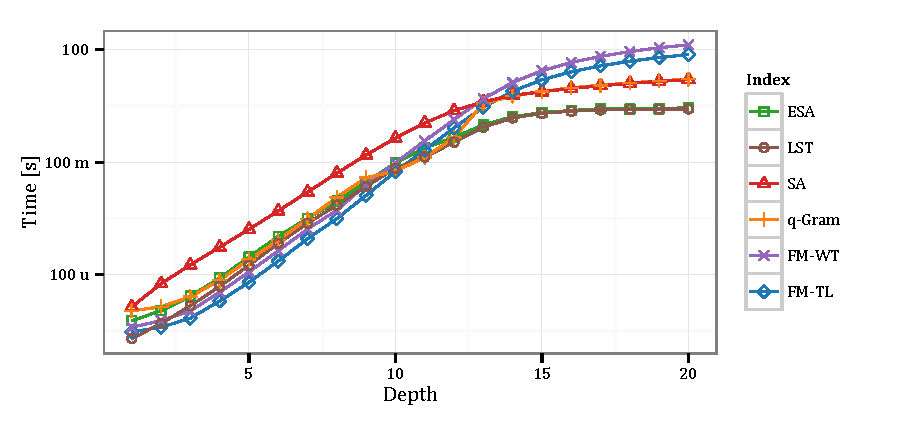
\includegraphics{visit.dna.celegans.pdf}
\end{center}
\end{figure}

\subsection{Exact string matching}
\label{sec:index:algo:exact}

I now give a simple algorithm performing exact string matching on a generic suffix trie.
In the following, I assume the text $t$ to be indexed by its suffix trie $\Ti$.
Algorithm~\ref{alg:st-exact} searches the pattern $p$ by starting in the root node of $\Ti$ and following the path spelling the pattern.
If the search ends up in a node $\Tn$, each leaf $\Ln_i$ below $\Tn$ points to a distinct suffix $t_{i..n}$ such that $t_{i..i+m}$ equals $p$.
%Algorithm~\ref{alg:st-exact} is correct since each path from the root to any internal node of the suffix trie $\Ti$ spells a different unique substring of $t$; consequently all equal substrings of $t$ are represented by a single common path.
If \textsc{goDown} is implemented in constant time and \textsc{occurrences} in linear time, all occurrences of $p$ into $t$ are found in optimal time $\Oh(m+o)$, where $m$ is the length of $p$ and $o$ its number of occurrences in $t$.

Figure \ref{fig:query-dna-exact} shows the results of the experimental evaluation of algorithm~\ref{alg:st-exact}.
On forward indices the search time becomes constant for patterns of length above 15, \ie when the index becomes sparse.
Conversely, on backward (FM) indices the search time is linear in the pattern length. 
The SA alone is at least 20\,\% slower than the $q$-gram index, hence never competitive.
In particular, the SA shows a runtime peak for patterns of length 10, due to the fact that binary search algorithms \ref{alg:sa-lower}--\ref{alg:sa-upper} converge more slowly for shorter patterns.
The ESA is never faster than the $q$-gram index despite its higher memory consumption.
Concerning FM-indices, the WT variant is almost twice as slow as the TL variant, as the WT-based rank dictionary performs twice the number of random memory accesses than the levels rank dictionary.
Summing up, the TL FM-index is the fastest index to match exact patterns within length 30, while the $q$-gram index is the fastest for patterns above length 30.
%Surprisingly, there is no clear time-memory tradeoff.

\begin{figure*}[b]
\begin{center}
\begin{minipage}[t]{.8\textwidth}
\begin{algorithm}[H]
\Algorithm{ExactSearch}{$t,p$}
\begin{tabular}{ll}
\textbf{Input}  & $t$ : pointer to the root node of the suffix trie of the text\\
				& $p$ : pointer to the pattern\\
\textbf{Output} & list of all occurrences of the pattern in the text\\
\end{tabular}
\begin{algorithmic}[1]
\If {\Call{atEnd}{$p$}}
	\State \Report \Call{occurrences}{$t$}
\ElsIf {\Call{goDown}{$t,\Call{value}{p}$}}
		\State {\Call{goNext}{$p$}}
		\State \Call{ExactSearch}{$t,p$}
\EndIf
\end{algorithmic}
\label{alg:st-exact}
\end{algorithm}
\end{minipage}
\end{center}
\end{figure*}

\begin{figure}[t]
\begin{center}
\caption[Exact string matching runtime]{Runtime of exact string matching on various suffix trie implementations.}
\label{fig:query-dna-exact}
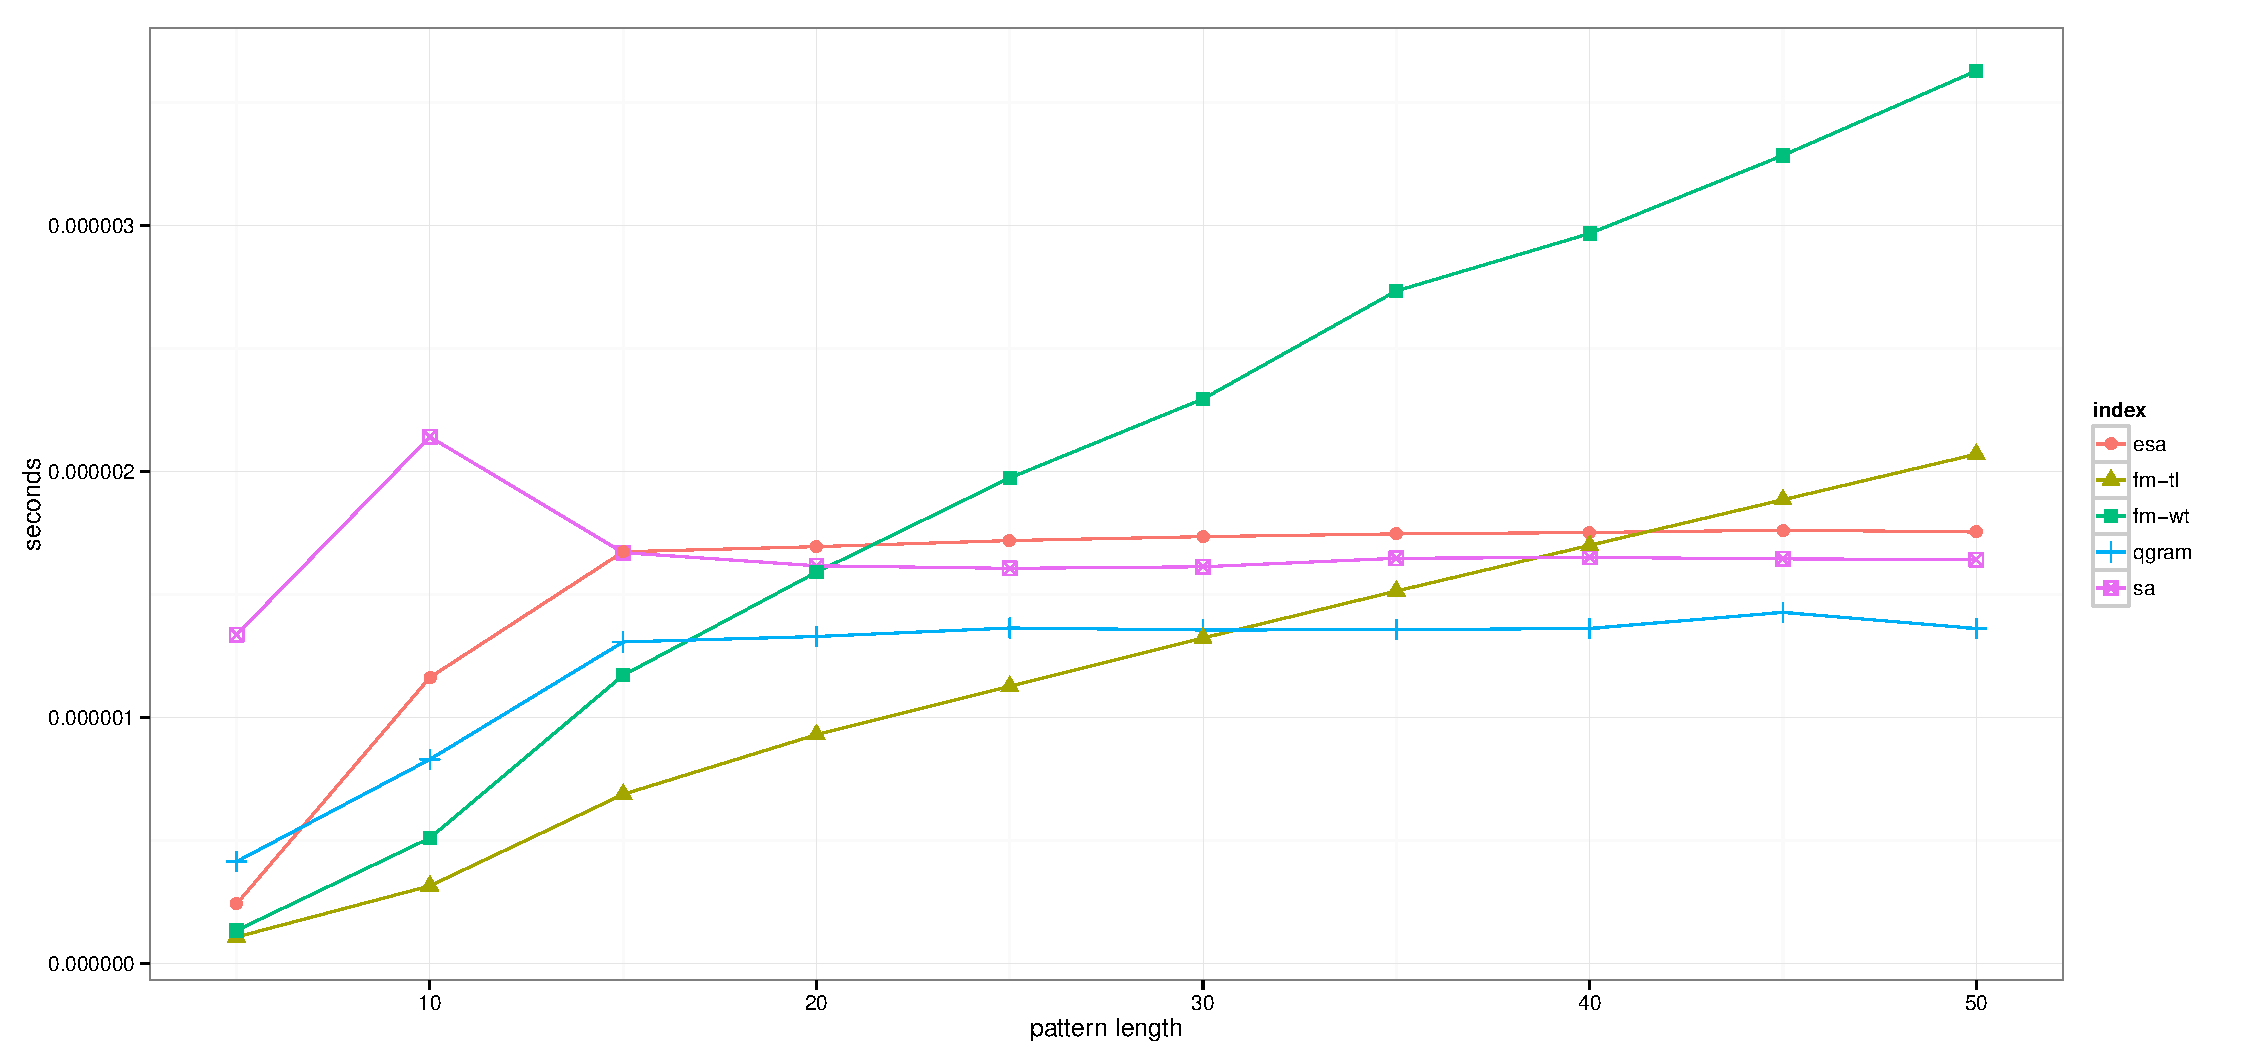
\includegraphics{query.dna.celegans.0.pdf}
\end{center}
\end{figure}

%\begin{figure}[h]
%\begin{center}
%\caption[Exact string matching on a suffix trie]{Exact string matching on a suffix trie. The pattern NA is searched exactly in the text ANANAS\$.}
%\label{fig:st-exact}
%\begin{tikzpicture}[scale=1.5,font=\sffamily]

\tikzstyle{level 1}=[sibling distance=12mm, level distance=6mm]
\tikzstyle{level 2}=[sibling distance=6mm, level distance=6mm]
\tikzstyle{level 3}=[sibling distance=6mm, level distance=6mm] 
\tikzstyle{level 4}=[sibling distance=6mm, level distance=6mm] 
\tikzstyle{level 5}=[sibling distance=6mm, level distance=6mm] 
\tikzstyle{level 6}=[sibling distance=6mm, level distance=6mm] 
\tikzstyle{level 7}=[sibling distance=6mm, level distance=6mm] 

%\tikzstyle{transparent}=[edge from parent/.style={draw=none}]
%\tikzstyle{el}=[->,thick,color=gray,text=mycolor1high]

\tikzstyle{transparent}=[edge from parent/.style={draw=none}]
\tikzstyle{el}=[->,thick,color=black,text=black]
\tikzstyle{inner}=[circle,draw,color=black,inner sep=1.5pt]

\node[inner](r) {}
child[transparent] {
node[leaf](D) {$7$}
}
child[transparent] {
node[inner](A) {}
child[transparent] {
node[inner](AN) {}
child[transparent] {
node[inner](ANA) {}
child[transparent] {
node[inner](ANAN) {}
child[transparent] {
node[inner](ANANA) {}
child[transparent] {
node[inner](ANANAS) {}
child[transparent] {
node[leaf](ANANASD) {$1$}
}
}
}
}
child[transparent] {
node[inner](ANAS) {}
child[transparent] {
node[leaf](ANASD) {$3$}
}
}
}
}
child[transparent] {
node[inner](AS) {}
child[transparent] {
node[leaf](ASD) {$5$}
}
}
}
child[transparent] {
node[inner](N) {}
child[transparent] {
node[inner](NA) {}
child[transparent] {
node[inner](NAN) {}
child[transparent] {
node[inner](NANA) {}
child[transparent] {
node[inner](NANAS) {}
child[transparent] {
node[leaf](NANASD) {$2$}
}
}
}
}
child[transparent] {
node[inner](NAS) {}
child[transparent] {
node[leaf](NASD) {$4$}
}
}
}
}
child[transparent] {
node[inner](S) {}
child[transparent] {
node[leaf](SD) {$6$}
}
}
;

\draw[el] (r) -- (D) \labelA{\$};
\draw[el] (r) -- (A) \labelA{A};
\draw[el] (A) -- (AN) \labelA{N};
\draw[el] (AN) -- (ANA) \labelA{A};
\draw[el] (ANA) -- (ANAN) \labelA{N};
\draw[el] (ANAN) -- (ANANA) \labelA{A};
\draw[el] (ANANA) -- (ANANAS) \labelA{S};
\draw[el] (ANANAS) -- (ANANASD) \labelA{\$};
\draw[el] (ANA) -- (ANAS) \labelA{S};
\draw[el] (ANAS) -- (ANASD) \labelA{\$};
\draw[el] (A) -- (AS) \labelA{S};
\draw[el] (AS) -- (ASD) \labelA{\$};

\draw[el] (r) -- (N) \labelA{N};
\draw[el] (N) -- (NA) \labelA{A};
\draw[el] (NA) -- (NAN) \labelA{N};
\draw[el] (NAN) -- (NANA) \labelA{A};
\draw[el] (NANA) -- (NANAS) \labelA{S};
\draw[el] (NANAS) -- (NANASD) \labelA{\$};
\draw[el] (NA) -- (NAS) \labelA{S};
\draw[el] (NAS) -- (NASD) \labelA{\$};
\draw[el] (r) -- (S) \labelA{S};
\draw[el] (S) -- (SD) \labelA{\$};

\end{tikzpicture}

%\end{center}
%\end{figure}

\subsection{Backtracking $k$-mismatches}
\label{sec:index:algo:kmismatches}

I now give an algorithm that solves $k$-mismatches by backtracking a generic suffix trie.
The idea of backtracking a suffix tree has been first proposed in \citep{Ukkonen1993}.
Recently, various popular bioinformatics tools \citep{Langmead2009, Li2009} adopted variations of this method in conjunction with a FM-index.
Yet, the idea dates back to more than twenty years ago.

\begin{figure*}[h!]
\begin{center}
\begin{minipage}[t]{.8\textwidth}
\begin{algorithm}[H]
\Algorithm{KMismatches}{$t,p,e$}
\begin{tabular}{ll}
\textbf{Input}  & $t$ : pointer to the root node of the suffix trie of the text\\
 			    & $p$ : pointer to the pattern\\
 			    & $e$ : integer bounding the number of mismatches\\
\textbf{Output} & list of all occurrences of the pattern in the text\\
\end{tabular}
\begin{algorithmic}[1]
\If {$e = k$}
	\State {\Call{ExactSearch}{$t,p$}}
\ElsIf {$e < k$}
	\If {\Call{atEnd}{$p$}}
		\State \Report \Call{occurrences}{$t$}
	\ElsIf {\Call{goDown}{$t$}}
		\Repeat
			\State {$d \gets \delta(\Call{label}{t}, \Call{value}{p})$}
			\State \Call{goNext}{$p$}
			\State \Call{KMismatches}{$t,p,e + d$}
			\State \Call{goPrevious}{$p$}
		\Until \Call{goRight}{$t$}
	\EndIf
\EndIf
\end{algorithmic}
\label{alg:st-hamming}
\end{algorithm}
\end{minipage}
\end{center}
\end{figure*}

Algorithm~\ref{alg:st-hamming} performs a top-down traversal on the suffix trie $\Ti$, spelling incrementally all distinct substrings of $t$.
While traversing each branch of the trie, this algorithm incrementally computes the distance between the query and the spelled string.
If the computed distance exceeds $k$, the traversal backtracks and proceeds on the next branch.
Conversely, if the pattern $p$ is completely spelled and the traversal ends up in a node $\Tn$, each leaf $\Ln_i$ below $\Tn$ points to a distinct suffix $t_{i..n}$ such that $d_H(t_{i..i+m}, p) \leq k$.

%The \emph{worst case} runtime of algorithm \ref{alg:st-hamming} is clearly independent of the text length $n$.
%According to \citep{Navarro2000}, this algorithm exhibits average time sublinear in $n$.

\begin{figure}[b]
\begin{center}
\caption[$k$-mismatches runtime]{Runtime of $1$-mismatch search on various suffix trie implementations.}
\label{fig:query-dna-apx}
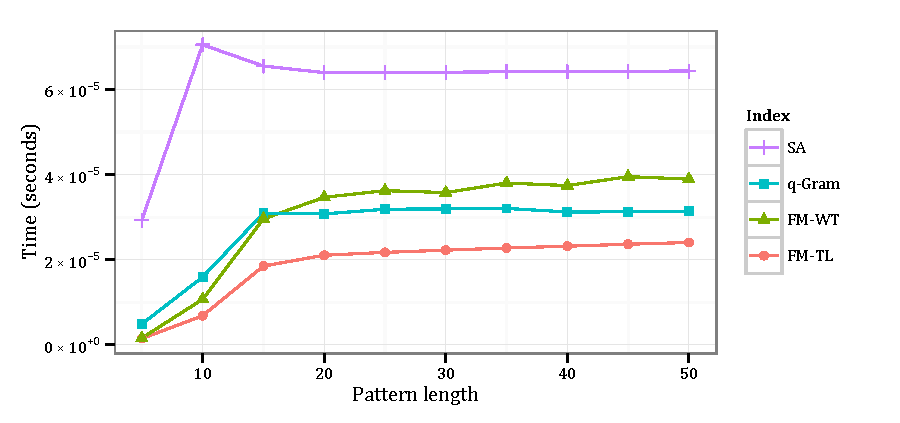
\includegraphics{query.dna.celegans.1.pdf}
\end{center}
\end{figure}

%\begin{figure}[h]
%\begin{center}
%\caption[Backtracking $k$-mismatches]{$k$-mismatches on a suffix trie.}
%\label{fig:st-hamming}
%\begin{tikzpicture}[scale=1.5,font=\sffamily]

\tikzstyle{level 1}=[sibling distance=12mm, level distance=6mm]
\tikzstyle{level 2}=[sibling distance=6mm, level distance=6mm]
\tikzstyle{level 3}=[sibling distance=6mm, level distance=6mm] 
\tikzstyle{level 4}=[sibling distance=6mm, level distance=6mm] 
\tikzstyle{level 5}=[sibling distance=6mm, level distance=6mm] 
\tikzstyle{level 6}=[sibling distance=6mm, level distance=6mm] 
\tikzstyle{level 7}=[sibling distance=6mm, level distance=6mm] 

%\tikzstyle{transparent}=[edge from parent/.style={draw=none}]
%\tikzstyle{el}=[->,thick,color=gray,text=mycolor1high]

\tikzstyle{transparent}=[edge from parent/.style={draw=none}]
\tikzstyle{el}=[->,thick,color=black,text=black]
\tikzstyle{inner}=[circle,draw,color=black,inner sep=1.5pt]

\node[inner](r) {}
child[transparent] {
node[leaf](D) {$7$}
}
child[transparent] {
node[inner](A) {}
child[transparent] {
node[inner](AN) {}
child[transparent] {
node[inner](ANA) {}
child[transparent] {
node[inner](ANAN) {}
child[transparent] {
node[inner](ANANA) {}
child[transparent] {
node[inner](ANANAS) {}
child[transparent] {
node[leaf](ANANASD) {$1$}
}
}
}
}
child[transparent] {
node[inner](ANAS) {}
child[transparent] {
node[leaf](ANASD) {$3$}
}
}
}
}
child[transparent] {
node[inner](AS) {}
child[transparent] {
node[leaf](ASD) {$5$}
}
}
}
child[transparent] {
node[inner](N) {}
child[transparent] {
node[inner](NA) {}
child[transparent] {
node[inner](NAN) {}
child[transparent] {
node[inner](NANA) {}
child[transparent] {
node[inner](NANAS) {}
child[transparent] {
node[leaf](NANASD) {$2$}
}
}
}
}
child[transparent] {
node[inner](NAS) {}
child[transparent] {
node[leaf](NASD) {$4$}
}
}
}
}
child[transparent] {
node[inner](S) {}
child[transparent] {
node[leaf](SD) {$6$}
}
}
;

\draw[el] (r) -- (D) \labelA{\$};
\draw[el] (r) -- (A) \labelA{A};
\draw[el] (A) -- (AN) \labelA{N};
\draw[el] (AN) -- (ANA) \labelA{A};
\draw[el] (ANA) -- (ANAN) \labelA{N};
\draw[el] (ANAN) -- (ANANA) \labelA{A};
\draw[el] (ANANA) -- (ANANAS) \labelA{S};
\draw[el] (ANANAS) -- (ANANASD) \labelA{\$};
\draw[el] (ANA) -- (ANAS) \labelA{S};
\draw[el] (ANAS) -- (ANASD) \labelA{\$};
\draw[el] (A) -- (AS) \labelA{S};
\draw[el] (AS) -- (ASD) \labelA{\$};

\draw[el] (r) -- (N) \labelA{N};
\draw[el] (N) -- (NA) \labelA{A};
\draw[el] (NA) -- (NAN) \labelA{N};
\draw[el] (NAN) -- (NANA) \labelA{A};
\draw[el] (NANA) -- (NANAS) \labelA{S};
\draw[el] (NANAS) -- (NANASD) \labelA{\$};
\draw[el] (NA) -- (NAS) \labelA{S};
\draw[el] (NAS) -- (NASD) \labelA{\$};
\draw[el] (r) -- (S) \labelA{S};
\draw[el] (S) -- (SD) \labelA{\$};

\end{tikzpicture}

%\end{center}
%\end{figure}

Figure \ref{fig:query-dna-apx} shows the results of the experimental evaluation of algorithm~\ref{alg:st-hamming} for $k=1$.
The TL FM-index is always faster than any other index: for instance, on patterns of length 30, the SA it is 3 times slower; even the $q$-gram index is 50\,\% slower than the TL FM-index.
On the TL FM-index, $1$-approximate matching of patterns of length 30 is 16 times slower than exact matching: on average, exact matching takes $1.3$ microseconds ($\mu s$), while $1$-approximate matching spends $21 \, \mu s$.

%\subsection{Backtracking $k$-differences}
%\label{sec:index:algo:kdifferences}
%
%I present two alternative algorithms for $k$-differences.
%Algorithm~\ref{alg:st-edit-explicit} explicitly enumerates errors while traversing the suffix trie. Conversely, algorithm~\ref{alg:st-edit} computes the edit distance between the pattern and any branch of the suffix trie.
%This latter algorithm necessitates of a method capable of checking incrementally whether the edit distance at any node is within the imposed threshold $k$.
%
%%Algorithm~\ref{alg:st-edit-explicit} reports more occurrences than algorithm~\ref{alg:st-edit}.
%%Discuss neighborhood, condensed neighborhood, and super-condensed neighborhood.
%%To obtain a better theoretical runtime, \citep{Navarro2000} consider an algorithm that computes in $\Oh(1)$ per node.
%
%\begin{figure*}[b]
%\begin{center}
%\begin{minipage}[t]{.8\textwidth}
%\begin{algorithm}[H]
%\Algorithm{KDifferences}{$t,p,e$}
%\begin{tabular}{ll}
%\textbf{Input}  & $t$ : pointer to the root node of the suffix trie of the text\\
% 			    & $p$ : pointer to the root node of the trie of the patterns\\
% 			    & $e$ : integer bounding the number of errors\\
%\textbf{Output} & list of all occurrences of the pattern in the text\\
%\end{tabular}
%\begin{algorithmic}[1]
%\If {$e = k$}
%	\State \Call{ExactSearch}{$t,p$}
%\Else
%	\State \Call{goNext}{$p$}
%	\State \Call{KDifferences}{$t,p,e+1$}
%	\State \Call{goPrevious}{$p$}
%	\If {\Call{goDown}{$t$}}
%		\Repeat
%			\State \Call{KDifferences}{$t,p,e+1$}
%			\State {$d \gets \delta(\Call{label}{t}, \Call{value}{p})$}
%			\State \Call{goNext}{$p$}
%			\State \Call{KDifferences}{$t,p,e + d$}
%			\State \Call{goPrevious}{$p$}
%		\Until {\Call{goRight}{$t$}}
%	\EndIf
%\EndIf
%\end{algorithmic}
%\label{alg:st-edit-explicit}
%\end{algorithm}
%\end{minipage}
%\end{center}
%\end{figure*}
%
%\begin{figure*}[b]
%\begin{center}
%\begin{minipage}[t]{.8\textwidth}
%\begin{algorithm}[H]
%\Algorithm{KDifferences}{$t,p,D$}
%\begin{tabular}{ll}
%\textbf{Input}  & $t$ : pointer to the root node of the suffix trie of the text\\
% 			    & $p$ : pointer to the root node of the trie of the patterns\\
% 			    & $D$ : vector of integers representing a DP column\\
%\textbf{Output} & list of all occurrences of the pattern in the text\\
%\end{tabular}
%\begin{algorithmic}[1]
%\If {$D[m] \leq k$}
%	\State \Report \Call{occurrences}{$t$}
%\ElsIf {$\min{D} \leq k$}
%	\If {\Call{goDown}{$t$}}
%		\Repeat
%			\State {$D' \gets$ \Call{DP}{$D, \Call{label}{t}, p$}}
%			\State \Call{goNext}{$p$}
%			\State \Call{KDifferences}{$t,p,D'$}
%			\State \Call{goPrevious}{$p$}
%		\Until {\Call{goRight}{$t$}}
%	\EndIf
%\EndIf
%\end{algorithmic}
%\label{alg:st-edit}
%\end{algorithm}
%\end{minipage}
%\end{center}
%\end{figure*}
%
%%\begin{algorithm}[h]
%%\caption{$k$-difference on a suffix trie.}
%%\label{alg:st-edit}
%%\begin{algorithmic}[1]
%%\Procedure{KDifferences}{$\Tn,p,e$}
%%	\ForAll {$\Cn \in \Ci(\Tn)$}
%%		\State \Call{KDifferences}{$\Cn,p_{2..|p|},e - d_E(repr(\Tn), p)$}
%%	\EndFor
%%\EndProcedure
%%\end{algorithmic}
%%\end{algorithm}


\subsection{Multiple exact string matching}
\label{sec:index:algo:multiexact}

Before turning to multiple $k$-mismatches, I describe a simpler algorithm for multiple exact string matching.
In addition to the text $t$, multiple exact string matching provides a collection of patterns $\mathbb{P}$.
Hence, in addition to the suffix trie $\mathcal{T}$ of $t$, algorithm \ref{alg:st-exact-multi} considers the trie $\mathcal{P}$ of $\mathbb{P}$.
Algorithm \ref{alg:st-exact-multi} matches simultaneously in $\mathcal{T}$ all patterns indexed in $\mathcal{P}$.
The traversal performed by algorithm \ref{alg:st-exact-multi} visits pairs of nodes in $\mathcal{T} \times \mathcal{P}$ whose entering edges have the same label.
Such traversal implicitly \emph{intersects} the two tries.
However, algorithm \ref{alg:st-exact-multi} is not symmetric: $\mathcal{T}$ and $\mathcal{P}$ cannot be interchanged.
The traversal stops whenever it reaches a leaf node in $\mathcal{P}$ and reports the occurrences pointed by all the leaves beneath the current node in $\mathcal{T}$.
%If the collection $\mathbb{P}$ contains two equal strings, some leaf of $\mathcal{P}$ points to more than one pattern.

\begin{figure*}[t]
\begin{center}
\begin{minipage}[t]{.8\textwidth}
\begin{algorithm}[H]
\Algorithm{MultipleExactSearch}{$t,p$}
\begin{tabular}{ll}
\textbf{Input}  & $t$ : pointer to the root node of the suffix trie of the text\\
 			    & $p$ : pointer to the root node of the trie of the patterns\\
\textbf{Output} & list of all occurrences of any pattern in the text\\
\end{tabular}
\begin{algorithmic}[1]
\If {\Call{isLeaf}{$p$}}
	\State \Report \Call{occurrences}{$t$} $\times$ \Call{occurrences}{$p$}
\Else
	\State \Call{goDown}{$p$}
	\Repeat
		\If {\Call{goDown}{$t, \Call{label}{p}$}}
			\State \Call{MultipleExactSearch}{$t,p$}
			\State \Call{goUp}{$t$}
		\EndIf
	\Until {\Call{goRight}{$p$}}
\EndIf
\end{algorithmic}
\label{alg:st-exact-multi}
\end{algorithm}
\end{minipage}
\end{center}
\end{figure*}

The experimental evaluation compares algorithm~\ref{alg:st-exact-multi} (Multiple) with algorithm~\ref{alg:st-exact} processing patterns in random order (Single) and in lexicographic order (Sorted).
Figure~\ref{fig:query-dna-exact-multi} shows the results.
In this evaluation, all patterns have length 15: runtimes shown in figure \ref{fig:query-dna-exact-multi} (histogram Single) correspond to runtimes shown in figure \ref{fig:query-dna-exact} (plots at pattern length 15).
%For instance, the indices ranked by query speed are: TL FM-index, WT FM-index, $q$-gram index, ESA and SA.

\begin{figure}[b]
\begin{center}
\caption[Multiple exact string matching runtime]{Runtime of multiple exact string matching on various suffix trie implementations. The preprocessing time is shown in black.}
\label{fig:query-dna-exact-multi}
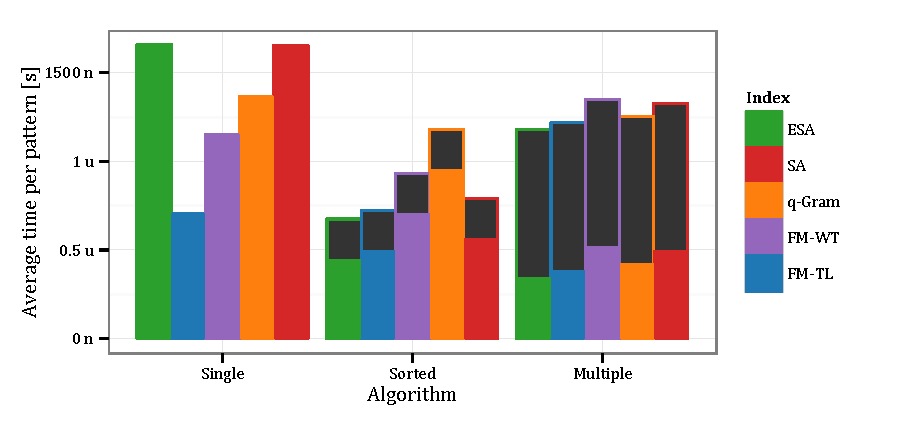
\includegraphics{multi.dna.celegans.0.15.pdf}
\end{center}
\end{figure}

Figure \ref{fig:query-dna-exact-multi} shows that a simple lexicographical sort of the patterns (histogram Sorted) speeds up algorithm \ref{alg:st-exact} on the SA and ESA by a factor of 2.
The same trick does not yield a significant speed-up on FM-indices nor on the $q$-gram index, as the $q$-gram directory already provides a cache local access pattern.

Algorithm~\ref{alg:st-exact-multi} (histogram Multiple) further reduces the traversal time.
Nonetheless, its runtime is dominated by the additional preprocessing time paid to construct the trie of the patterns.
This algorithm becomes more useful within the multiple $k$-mismatches algorithm.

\subsection{Multiple $k$-mismatches}
\label{sec:index:algo:multimismatch}

Algorithm \ref{alg:st-hamming-multi} receives a collection of patterns $\mathbb{P}$ and performs multiple $k$-mismatches using the associated trie $\mathcal{P}$.

The experimental evaluation compares algorithm~\ref{alg:st-hamming-multi} (Multiple) with algorithm~\ref{alg:st-hamming} processing patterns in random order (Single) and in lexicographic order (Sorted).
In this evaluation, all patterns have length 30: runtimes shown in figure \ref{fig:query-dna-apx-multi} (histogram Single) correspond to runtimes shown in figure \ref{fig:query-dna-apx} (plots at pattern length 30).

Algorithm \ref{alg:st-hamming} on lexicographically sorted patterns (histogram Sorted) is faster by a factor of 2 or more, on all indices.
The time to sort the patterns becomes insignificant compared to the traversal time.
Algorithm \ref{alg:st-exact-multi} (histogram Multiple) reduces traversal time by a factor 5 on SA and ESA, thus the time to construct the trie of the patterns is easily justified.
In practice, algorithm \ref{alg:st-exact-multi} fills the gap between the runtime of the SA and the $q$-gram index.
Surprisingly, algorithm \ref{alg:st-exact-multi} increases traversal time on FM-indices.

\begin{figure*}[b]
\begin{center}
\begin{minipage}[t]{.8\textwidth}
\begin{algorithm}[H]
\Algorithm{MultipleKMismatches}{$t,p,e$}
\begin{tabular}{ll}
\textbf{Input}  & $t$ : pointer to the root node of the suffix trie of the text\\
 			    & $p$ : pointer to the root node of the trie of the patterns\\
 			    & $e$ : integer bounding the number of mismatches\\
\textbf{Output} & list of all occurrences of any pattern in the text\\
\end{tabular}
\begin{algorithmic}[1]
\If {$e = k$}
	\State {\Call{MultipleExactSearch}{$t,p$}}
\ElsIf {$e < k$}
	\If {\Call{isLeaf}{$p$}}
		\State \Report \Call{occurrences}{$t$} $\times$ \Call{occurrences}{$p$}
	\ElsIf {\Call{goDown}{$t$}}
		\Repeat
			\State {\Call{goDown}{$p$}}
			\Repeat
				\State {$d \gets \delta(\Call{label}{t}, \Call{label}{p})$}
				\State \Call{MultipleKMismatches}{$t,p,e+d$}
			\Until {\Call{goRight}{$p$}}
			\State {\Call{goUp}{$p$}}
		\Until {\Call{goRight}{$t$}}
	\EndIf
\EndIf
\end{algorithmic}
\label{alg:st-hamming-multi}
\end{algorithm}
\end{minipage}
\end{center}
\end{figure*}

\begin{figure}[b]
\begin{center}
\caption[Multiple $k$-mismatches runtime]{Runtime of multiple $k$-mismatches on various suffix trie implementations. The preprocessing time is shown in black.}
\label{fig:query-dna-apx-multi}
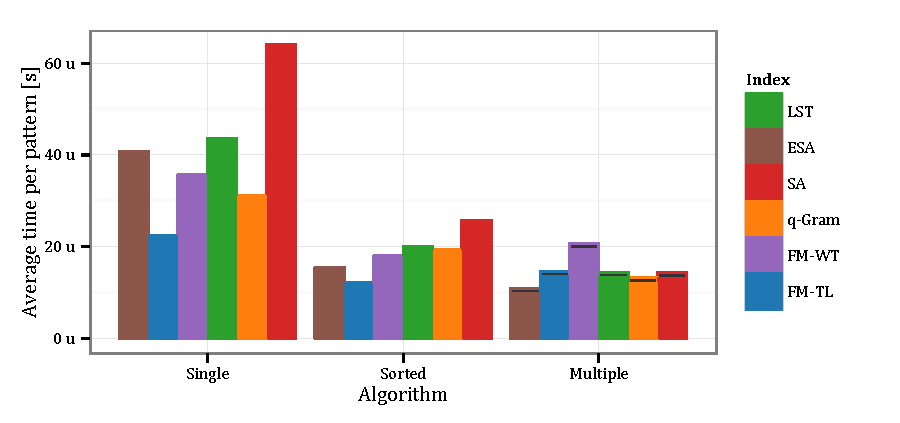
\includegraphics{multi.dna.celegans.1.30.pdf}
\end{center}
\end{figure}

